\section{Related Work}
\label{sec:related_work}
In this section, we review three sets of related work: data-driven methods, coupling learning and attention-based relation modeling, and multi-component fusion for traffic prediction.

\subsection{Data-driven traffic prediction}
Compared to knowledge-driven methods using queuing theory such as in \cite{cascetta2013transportation}, data-driven methods have dominated the recent traffic forecasting research, benefiting from the convenient acquisition of a huge amount of traffic data and the vigorous development of machine learning models. The early work on data-driven traffic forecasting mostly focuses on time series analysis, such as ARIMA \cite{williams2003modeling} and VAR \cite{zivot2006vector}, which typically rely on the stationarity assumption. To eliminate this assumption, recent research shifts to deep-learning-based models. Various efforts, e.g., \cite{zhao2017lstm,ma2015long,bai2020adaptive,pan2020spatio}, applied RNN and its variants such as LSTM \cite{hochreiter1997long} and GRU \cite{cho2014learning} to learn relations in traffic data automatically, taking advantage of the RNN’s superior ability in modeling the temporal dynamics in time series data \cite{connor1994recurrent}. However, they overlook other relations such as the spatial relations. Accordingly, other attempts based on deep learning for traffic forecasting (e.g., \cite{wu2016short,ma2017learning,zhang2017deep}) deployed CNN to pay more attention to spatial relations among the traffic series from different traffic nodes. However, due to the fact that CNN is preferable to manipulating regular grid data (e.g., 2D images), those CNN methods force the spatial structure among different traffic series into a Euclidean space which is naturally violated by real-world traffic data. Considering the structural characteristics of traffic data, more recent work leverages the GNN (e.g., GCN \cite{kipf2016semi}, a special kind of CNN generalized for graph-structured data) to model the spatial relations in traffic road networks. For example, STGCN \cite{yu2017spatio} formulates the traffic prediction problem as graphs instead of applying regular recurrent and convolutional neural units in a deep learning architecture. In the same manner, DCRNN \cite{li2017diffusion}, Graph WaveNet \cite{wu2019graph} and GSTNet \cite{fang2019gstnet} utilized various GCNs to capture the prominent spatial interactions among different traffic series. Their efforts gain the state-of-the-art performance, thus opening a new door for traffic prediction. In contrast, our work in this paper is also based on GCN (\cite{mengzhang2020spatial, song2020spatial}) to model a traffic system as a spatio-temporal graph. We pay attention not only to the different relations embedded in a graph structure but also to their coupling strengths with each other. Our method innovatively models the traffic signals-based channel relations indispensable and hidden in a dynamic evolving systems like road  networks. This channel relation modeling complements with the spatio-temporal prediction for capturing more comprehensive traffic conditions. Note that the traffic data we discuss in this paper refers to the readings of traffic signals acquired by a variety of geo-sensors in a traffic road network, e.g., traffic flow or speed. 

\subsection{Coupling learning and attention-based relation modeling}
Complex systems like traffic networks are embedded with hierarchical and heterogneous coupling relationships and interactions within and between entities, subsystems and systems. Coupling learning captures the relationships and interactions in various settings, \cite{Huaaai19,2018CoupledCF}. They involve various techniques including incorporating metric learning, representation learning, multikernel learning, coupled hidden markov models and deep neural networks into modeling complex couplings and interactions\footnote{Interested readers may find more in https://datasciences.org/coupling-learning/.}. This paper expands coupling learning to learn multi-aspect traffic signal couplings by treating a traffic system as a coupled traffic network.

The attention mechanism is initially used in neural machine translation tasks \cite{bahdanau2014neural}. Its core idea is to adaptively pick up features that are relatively critical to specific tasks by learning the relations hidden inside input data. In recent years, it has been widely applied in various sequence-to-sequence (seq2seq) issues, such as air quality forecasting \cite{cheng2018neural} and sequential recommendation \cite{2018CoupledCF}. Typically, self-attention \cite{vaswani2017attention, velivckovic2017graph}  has been applied in traffic prediction to  model dependencies, as shown in traffic prediction models like GeoMAN \cite{liang2018geoman} using a multi-level attention-based recurrent neural network to predict the readings of a geo-sensor over several future hours and ASTGCN \cite{guo2019attention} implementing an attention-based spatial-temporal graph convolutional network for traffic flow forecasting. GMAN \cite{zheng2020gman} proposes a graph multi-attention network in an encoder-decoder architecture to carry out long-term traffic prediction. All the attention-based prediction models (e.g., \cite{liang2018geoman, guo2019attention, zheng2020gman, cai2020traffic, fang2020constgat, park2020st, chen2020multi}) tend to improve the effect of capturing spatio-temporal dependencies by leveraging self-attention to cooperate with the related convolutional operations. However, considering that the input and output of a self-attention module are generally two sequences of vectors, existing prediction models either develop self-attention separately in the spatial dimension of traffic conditions or in its temporal dimension, and thus they can not be easily deployed in a multi-dimensional information space. Even if their self-attention processes are stubbornly implemented on each dimension of multi-dimensional input data in turn, the resultant model will fall into such dilemmas of a large parameter scale and the code-level redundancy. To this end, we aim to synchronously capture several sorts of significant relations among multi-dimensional traffic data. Thus, a multi-dimensional self-attention scheme is proposed to universally and conveniently model different information dimensions of input data with less computational and development costs.

\begin{figure*}[!ht]
    \centering
    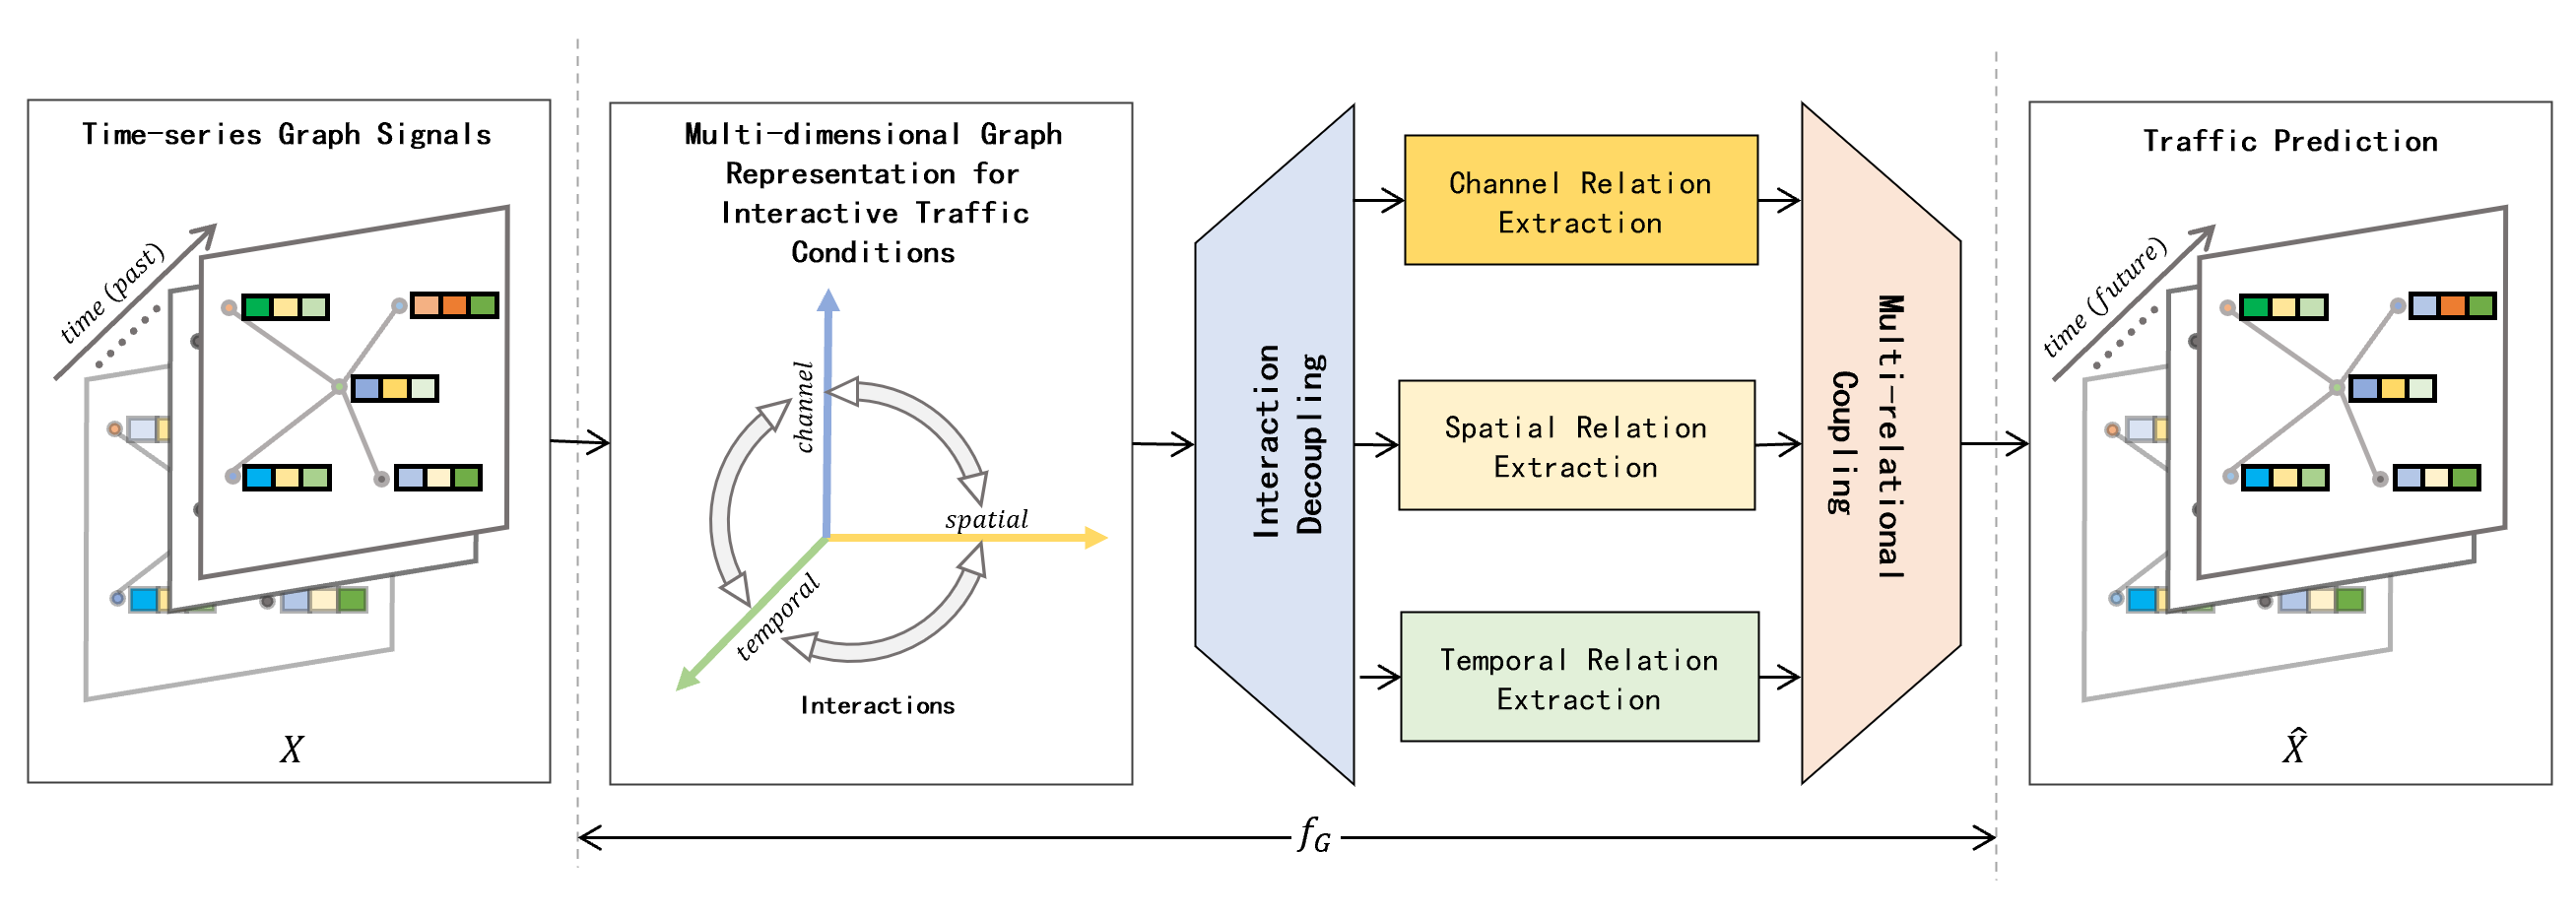
\includegraphics[width=0.9\textwidth]{pictures/Core.png}
    \caption{The framework of modeling spatio-temporal traffic signal coupling relationships from multiple channels in a dynamic traffic system. It forms a three-dimensional graph representation of interactive traffic conditions and further provides a multi-relational view of traffic prediction, where the temporal, spatial and channel relations are explicitly and implicitly coupled in the entire evolving traffic network. Our method firstly decouples them for separate representations and then couples their representations to formulate a multi-relational traffic graph.}
    \label{fig:core}
\end{figure*}


\subsection{Multi-component fusion}
The idea of multi-component fusion originates from ensemble learning \cite{dong2020survey}. In ITS, a few studies have leveraged the multi-component architectural style to deploy specific learning models for various tasks. For instance, \cite{geng2019spatiotemporal} shows a novel deep learning model  ST-MGCN for ride-hailing demand forecasting. For forecasting traffic flow in a road network, ASTGCN \cite{guo2019attention} enjoys a great success by adopting a gated mechanism based on time embedding to fuse multiple components. In contrast, our method MS-GAT also involves the multi-component fusion by using a time-gated mechanism for traffic prediction, it is more flexible in the preparation of training samples, which is crucial to the final performance and generalization capability of a supervised learning model. Specifically, instead of fixing the input sequence of each component by intuitively judging the importance of the chosen input sequence (e.g., \cite{guo2019attention}), our multi-component fusion design can provide richer and more diverse time-series graph data for the supervised learning according to the genuine importance of the input time-series graph data of each component to the same output sequence. In other words, our design is equipped with an effective data augmentation scheme, which can make full use of all the observed data along the time-axis to pick up their latent patterns sensitive to prediction.

